\documentclass[11pt]{article}
\usepackage[margin=1in]{geometry}
\usepackage{booktabs}
\usepackage{pgfplots}
\pgfplotsset{compat=1.18}
\usepackage{lipsum}
\usepackage{hyperref}

\title{Measuring Widgets: A Demonstration Paper}
\author{latex-diff-viewer demo}
\date{2026}

\begin{document}
\maketitle

\begin{abstract}
This short, multi-page paper exists to demonstrate \texttt{latex-diff-viewer}.
Browse the diffs between its commits to see added text in blue and removed text
struck through, and click a changed page to jump straight to it.
\end{abstract}

\section{Introduction}
\lipsum[1-2]

\section{Results}
\lipsum[3]

\begin{table}[t]
  \centering
  \begin{tabular}{lrr}
    \toprule
    Method   & Throughput & Latency \\
    \midrule
    Baseline & 100        & 12      \\
    Ours     & 145        & 9       \\
    \bottomrule
  \end{tabular}
  \caption{Widget throughput and latency.}
  \label{tab:results}
\end{table}

\lipsum[4-5]

\section{Method}
\lipsum[6]

\begin{figure}[t]
  \centering
  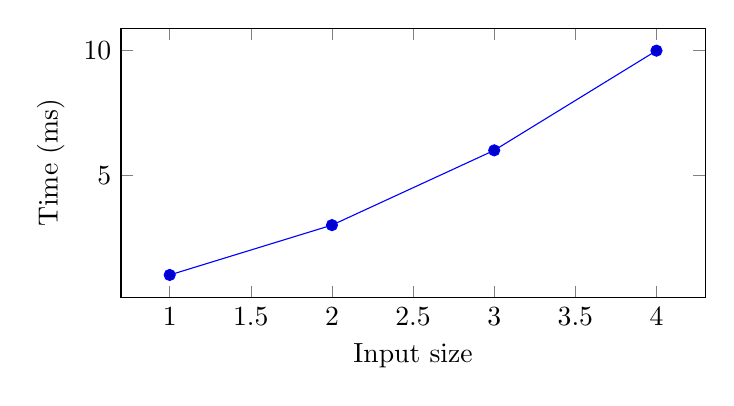
\begin{tikzpicture}
    \begin{axis}[width=9cm, height=5cm, xlabel=Input size, ylabel=Time (ms)]
      \addplot coordinates {(1,1) (2,3) (3,6) (4,10)};
    \end{axis}
  \end{tikzpicture}
  \caption{Time versus input size.}
  \label{fig:scaling}
\end{figure}

\lipsum[7-8]

\section{Conclusion}
\lipsum[9]

\end{document}
